%%%%%%%%%%%%%%%%%%%%%%%%%%%%%%%%%%%%%%%%%
% Beamer Presentation
% LaTeX Template
% Version 1.0 (10/11/12)
%
% This template has been downloaded from:
% http://www.LaTeXTemplates.com
%
% License:
% CC BY-NC-SA 3.0 (http://creativecommons.org/licenses/by-nc-sa/3.0/)
%
%%%%%%%%%%%%%%%%%%%%%%%%%%%%%%%%%%%%%%%%%

%----------------------------------------------------------------------------------------
%	PACKAGES AND THEMES
%----------------------------------------------------------------------------------------

\documentclass[hideothersubsections]{beamer}

\newcommand\parallelcontent[2]{
	\begin{columns}[t]
		\column{0.48\textwidth} #1
		\column{0.48\textwidth} #2
	\end{columns}
}
\newcommand\parallelitem[2]{
	\parallelcontent
	{\begin{itemize} \item #1 \end{itemize}}
	{\begin{itemize} \item #2 \end{itemize}}
}

\mode<presentation> {

% The Beamer class comes with a number of default slide themes
% which change the colors and layouts of slides. Below this is a list
% of all the themes, uncomment each in turn to see what they look like.

%\usetheme{default}
%\usetheme{AnnArbor}
%\usetheme{Antibes}
%\usetheme{Bergen}
%\usetheme{Berkeley}
%\usetheme{Berlin}
%\usetheme{Boadilla}
%\usetheme{CambridgeUS}
%\usetheme{Copenhagen}
%\usetheme{Darmstadt}
%\usetheme{Dresden}
%\usetheme{Frankfurt}
%\usetheme{Goettingen}
%\usetheme{Hannover}
%\usetheme{Ilmenau}
%\usetheme{JuanLesPins}
%\usetheme{Luebeck}
%\usetheme{Madrid}
%\usetheme{Malmoe}
%\usetheme{Marburg}
%\usetheme{Montpellier}
\usetheme{PaloAlto}
%\usetheme{Pittsburgh}
%\usetheme{Rochester}
%\usetheme{Singapore}
%\usetheme{Szeged}
%\usetheme{Warsaw}

% As well as themes, the Beamer class has a number of color themes
% for any slide theme. Uncomment each of these in turn to see how it
% changes the colors of your current slide theme.

%\usecolortheme{albatross}
%\usecolortheme{beaver}
%\usecolortheme{beetle}
%\usecolortheme{crane}
%\usecolortheme{dolphin}
%\usecolortheme{dove}
%\usecolortheme{fly}
%\usecolortheme{lily}
%\usecolortheme{orchid}
%\usecolortheme{rose}
%\usecolortheme{seagull}
\usecolortheme{seahorse}
%\usecolortheme{whale}
%\usecolortheme{wolverine}

%\setbeamertemplate{footline} % To remove the footer line in all slides uncomment this line
%\setbeamertemplate{footline}[page number] % To replace the footer line in all slides with a simple slide count uncomment this line

%\setbeamertemplate{navigation symbols}{} % To remove the navigation symbols from the bottom of all slides uncomment this line
}
\usefonttheme[onlysmall]{structurebold}
\usepackage{graphicx} % Allows including images
\usepackage{booktabs} % Allows the use of \toprule, \midrule and \bottomrule in tables

%----------------------------------------------------------------------------------------
%	TITLE PAGE
%----------------------------------------------------------------------------------------

\title[]{Theoretical and Numerical Studies of Efimov States} % The short title appears at the bottom of every slide, the full title is only on the title page

\author{Kajsa-My Blomdahl} % Your name
\institute[SU] % Your institution as it will appear on the bottom of every slide, may be shorthand to save space
{
Stockholms Universitet \\ % Your institution for the title page
\medskip
\textit{kajsamy.blomdahl@fysik.su.se} % Your email address
}
\date{\today} % Date, can be changed to a custom date
%\logo{
\includegraphics[height=1.0cm]{logga}}

%\AtBeginSubsection[]
%{
%	\begin{frame}
%	\frametitle{Table of Contents}
%	\tableofcontents[currentsection,currentsubsection]
%\end{frame}
%}

\begin{document}
	
\begin{frame}
	\titlepage
\end{frame}

\section[Outline]{}
\frame{\tableofcontents}

%----------------------------------------------------------------------------------------
%	PRESENTATION SLIDES
%----------------------------------------------------------------------------------------
\section{Introduction}
\subsection{Background}
\begin{frame}
\frametitle{Efimov's Prediction}
\begin{itemize}
	\item Resonant 2-body forces can give rise to a series of bound energy levels in 3-particle systems.
	\item When the short-ranged two-body forces approached resonance, he found a universal long-range three-body attraction emerging, giving rise to an infinite number of trimer states with binding energies obeying a discrete scaling law at resonance.
	
\end{itemize}
\end{frame}

%-----------------------------------------------

\begin{frame}
\frametitle{The Peculiar Efimov Effect}
\begin{itemize}
\item The size of each Efimov state is much larger than the force-range between the individual particle pairs $\rightarrow$ quantum mechanical state.
\item When the 2B s-wave scattering length $a \rightarrow \pm\infty$ the $\#$ of bound states is infinite.
\item  $\#$ of 3B bound states is \textit{reduced} as the 2B interaction is made more attractive.
\item Emerge irrespective of the nature of the 2B forces and can \textit{in principle} be observed in all quantum mechanical systems. 
\end{itemize}
\end{frame}

%------------------------------------------------

\subsection{Scattering length}
\begin{frame}
\frametitle{Scattering Length}
\begin{itemize}
	\item The 2B $s$-wave scattering length characterise the strength of the interparticle interaction. Definition:
	\begin{equation}
	a = \lim_{k \to 0} -\frac{\tan\delta_0(k)}{k}
	\end{equation}
	\item Negative scattering lengths correspond to an attractive effective interaction.
	\item Positive scattering lengths correspond to a repulsive effective interaction.
\end{itemize}
\end{frame}

\subsection{Universality}
\begin{frame}
\frametitle{Universality In 2B Systems}
\begin{block}{2B Scattering}
	Particles with large scattering lengths in the low-energy regime have universal properties. 
\end{block}

\begin{block}{Universal Properties.. In What Sense?}
	Depend on the scattering length alone and not on the details of the short-range interaction.
\end{block}

\begin{block}{Exemple: 2B Binding Energy For 2 Identical Bosons}
	\begin{equation}
	E_D = \frac{\hbar^2}{2 \mu_{2b} a^2}.
	\end{equation}
\end{block}
\end{frame}

\begin{frame}
\frametitle{Universality in 3B Systems}
\begin{figure}
	\centering
	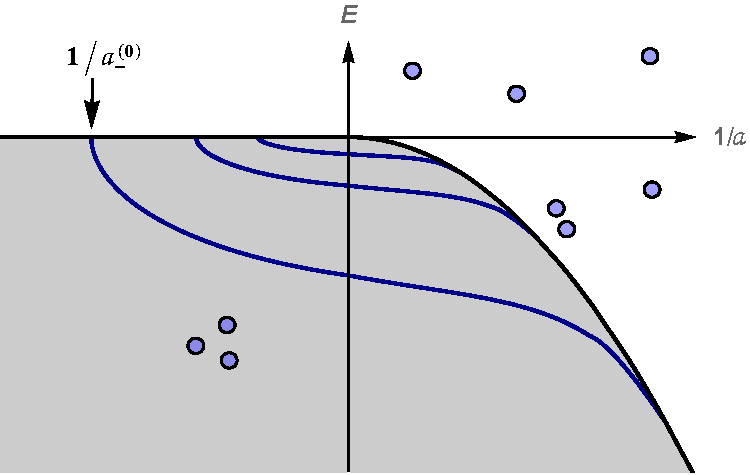
\includegraphics[width=0.5\linewidth]{efimov_spec}
	\caption{The energies of the three first Efimov states are plotted as functions of the inverse scattering length $a$. Three different regions can be identified in the figure.	The energy levels scale geometrically: $\frac{E_T^{n+1}}{E_T^{n}} = e^{2\pi/s_0} \approx 515$, for identical bosons ($s_0 \simeq 1.00624$ for $J=0^+$ states).}
\end{figure} 
\end{frame}

\section{Solving The 3-body Problem; Theoretical approach}
\begin{frame}
\frametitle{3-Particles, What Is The Problem?!}
\begin{block}{Apparently simple, However}
	\begin{itemize}
	\item The configuration space for the 3BP is 6D after separating out the center of mass motion.
	\item 3 additional constants of motion can be provided by conservation of the total angular momentum.
	\item This leaves a three dimensional Schr{\"o}dinger equation in the quantum case.
	\end{itemize}
\end{block}
\end{frame}

\subsection{Step 1: Introduce Jacobi Coordinates}
\begin{frame}
\frametitle{Jacobi Coordinates}
\begin{figure}
\centering
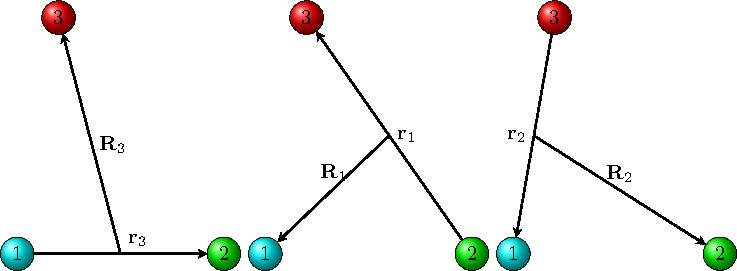
\includegraphics[width=0.7\linewidth]{jacobi.pdf}
%\caption{Spatial positions of three particles.}
\end{figure}
\end{frame}

\begin{frame}
\frametitle{Solving The 3-body Problem: Step 2, Hyperspherical Coordinates}
\begin{itemize}
	\item Separate internal and external coordinates
	\item Internal coordinates: 1 hyperradius: controls the size 
	\item Internal coordinates: 2 hyperangles: shape and particle permutations
\end{itemize}
\end{frame}

\begin{frame}[label=supplemental]
\frametitle{Solving The 3-body Problem: Step 3, Adiabatic Representation}
The Schr{\"o}dinger equation in hyperspherical coordinates
\begin{equation}
\bigg(-\frac{1}{2 \mu}\frac{\partial^2}{\partial \rho^2} + \frac{ \Lambda^2 + \frac{15}{4}}{2 \mu \rho^{2}}+ V(\rho,\Omega)\bigg)\psi(\rho,\Omega) = E\psi(\rho,\Omega).
\end{equation}

\begin{itemize}
\item Treat the hyperradius as a parameter! 

\item $\rightarrow$ 3-body Born-Oppenheimer-like potential
\end{itemize}
\begin{equation}\label{adiabatic}
H_{ad}\Phi_{\nu}{(\rho;\Omega)} = U_{\nu}{(\rho)}\Phi_{\nu}(\rho;\Omega)
\end{equation}
\hyperlink{matrix}{\beamerbutton{Numerical Approach}}
\end{frame}

%------------------------------------

\begin{frame}
\frametitle{Solving The 3-body Problem: Step 4, 3-Body Energies}
The total wave function, 

\begin{equation}\label{wave}
\psi_{n}(\rho,\Omega) = \sum_{\nu=0}^{\infty} F_{n\nu}(\rho)\Phi_{\nu}(\rho;\Omega),
\end{equation}
can in this way be represented in terms of adiabatic states, which, in principle, yields an exact representation of the three-body Schr{\"o}dinger equation if all couplings are included.
\end{frame}

\begin{frame}
\frametitle{Solving The 3-body Problem: Step 4, Continued}
\begin{align}\label{fullhamiltonian}
\bigg(-\frac{1}{2 \mu}\frac{\partial^2}{ \partial \rho^2} + U_{\mu}(\rho) - \frac{1}{2\mu}Q_{\mu\mu}(\rho) \bigg)F_{n\mu}(\rho)&\nonumber\\ -\frac{1}{2\mu}\bigg(\sum_{\nu\neq\mu}2P_{\mu\nu}(\rho)\frac{\partial}{\partial\rho} + Q_{\mu\nu}(\rho) \bigg)F_{n\nu}(\rho)& = E_nF_{n\mu}(\rho).
\end{align}
\end{frame}

\section{Effective Potentials}
\subsection{The General Form}
\begin{frame}
\frametitle{Emergent Attractive and Repulsive Potentials}
In the adiabatic approximation the effective potentials are defined as 

\begin{equation}
W_{\nu}(\rho) = U_{\nu}(\rho)-\frac{1}{2\mu}Q_{\nu \nu}(\rho) = U_{\nu}(\rho)-\frac{1}{2\mu}P_{\nu \nu}^2(\rho).
\end{equation} 
These potentials are used for determining the single channel solutions of \eqref{fullhamiltonian}. 
\end{frame}

%------------------------------------------------------

\subsection{Convergence In the Asymptotic Limit}
\begin{frame}
\frametitle{Convergence In the Asymptotic Limit}
\begin{columns}
\column{0.46\textwidth}
\vskip-45pt
\visible<1-4>{\begin{block}{For $a<0$:}
		\begin{equation*}
		W_{\nu}(\rho) \xrightarrow{ \rho \to \infty}\frac{\lambda(\lambda+4)+\frac{15}{4}}{2\mu \rho^2}
		\end{equation*}
\end{block}
\vspace{1.35cm}}
\visible<3-4>{\begin{block}{For $a>0$:}
		\begin{equation*}
		W_{\nu}(\rho) \xrightarrow{ \rho \to \infty} E_{2b} +\frac{l(l+1)}{2\mu \rho^2}
		\end{equation*}
	\end{block}}
\column{0.54\textwidth}
\raggedright
\visible<2-4>{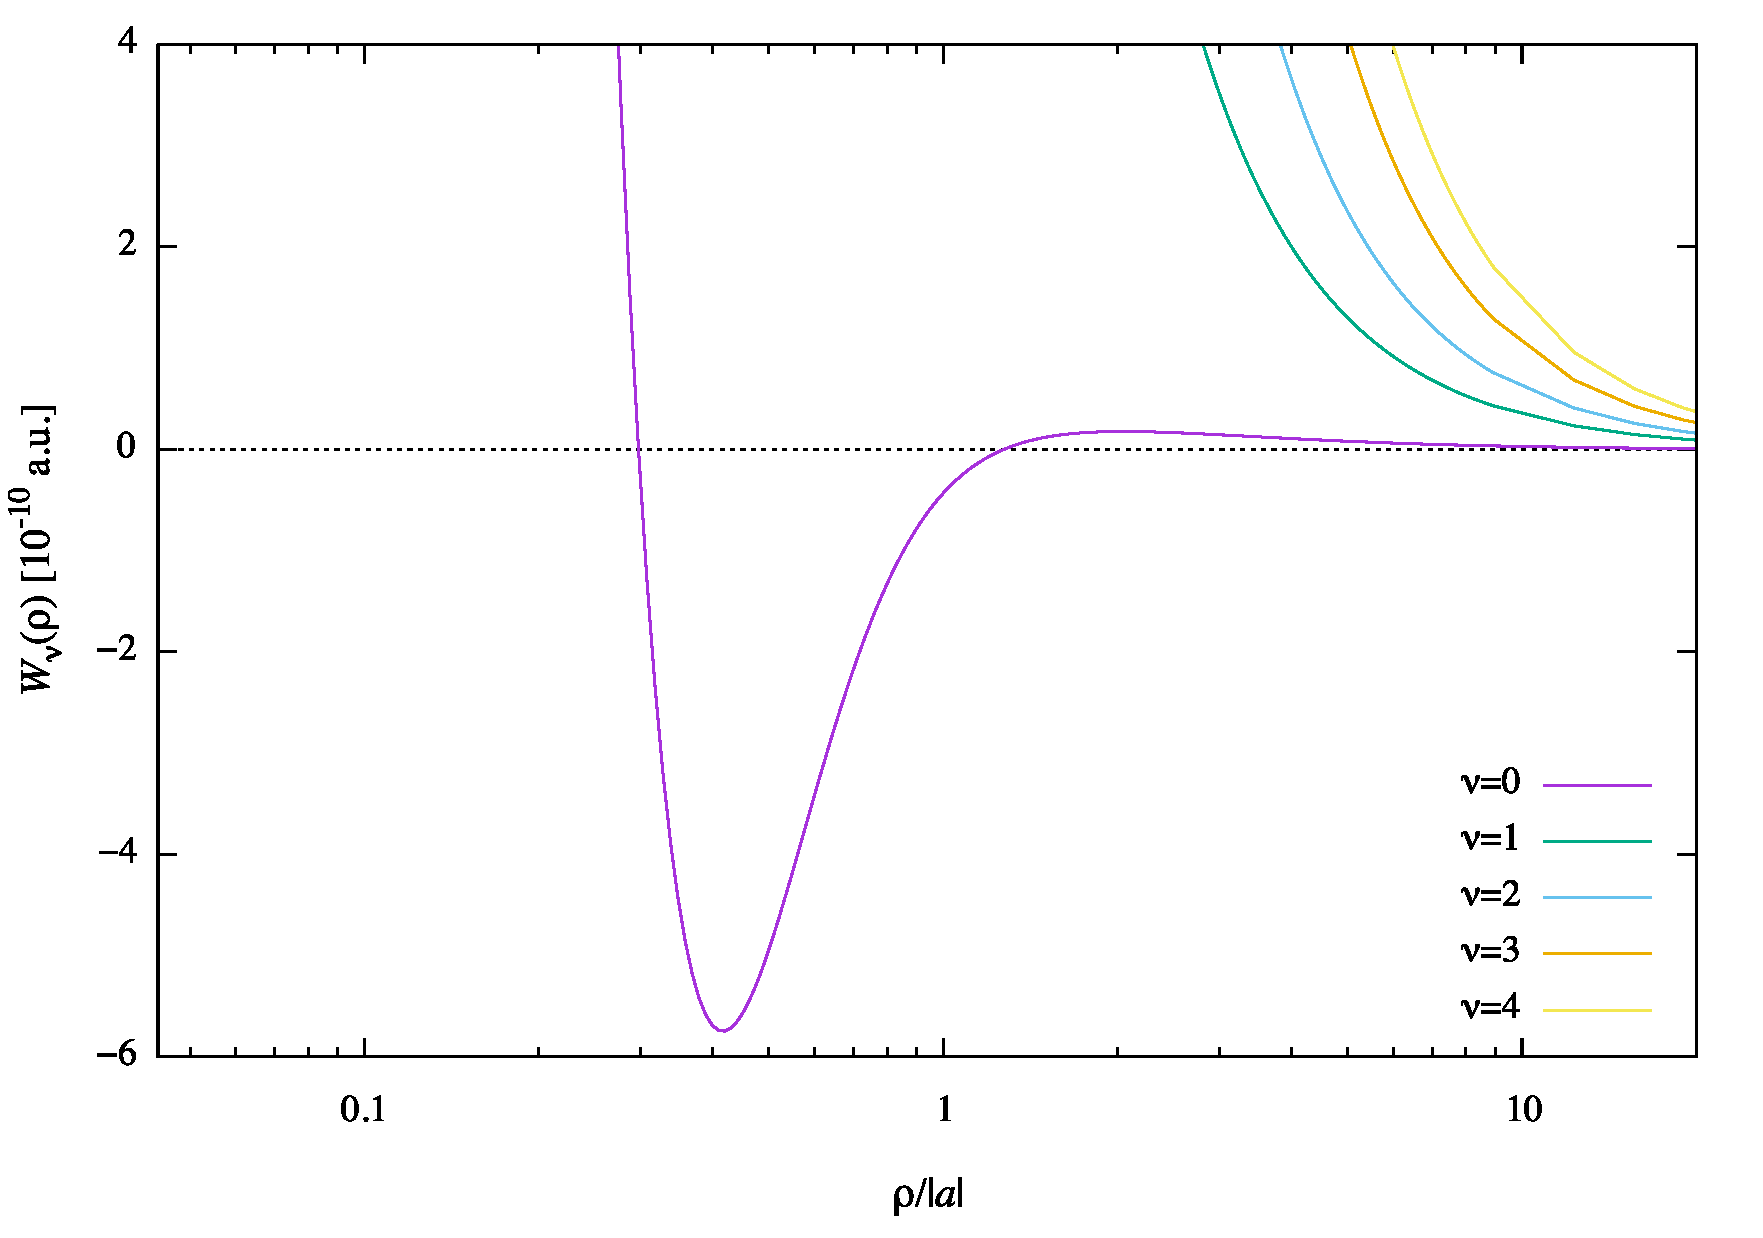
\includegraphics[width=1.0\linewidth]{Wneg.pdf}\\}
\visible<4>{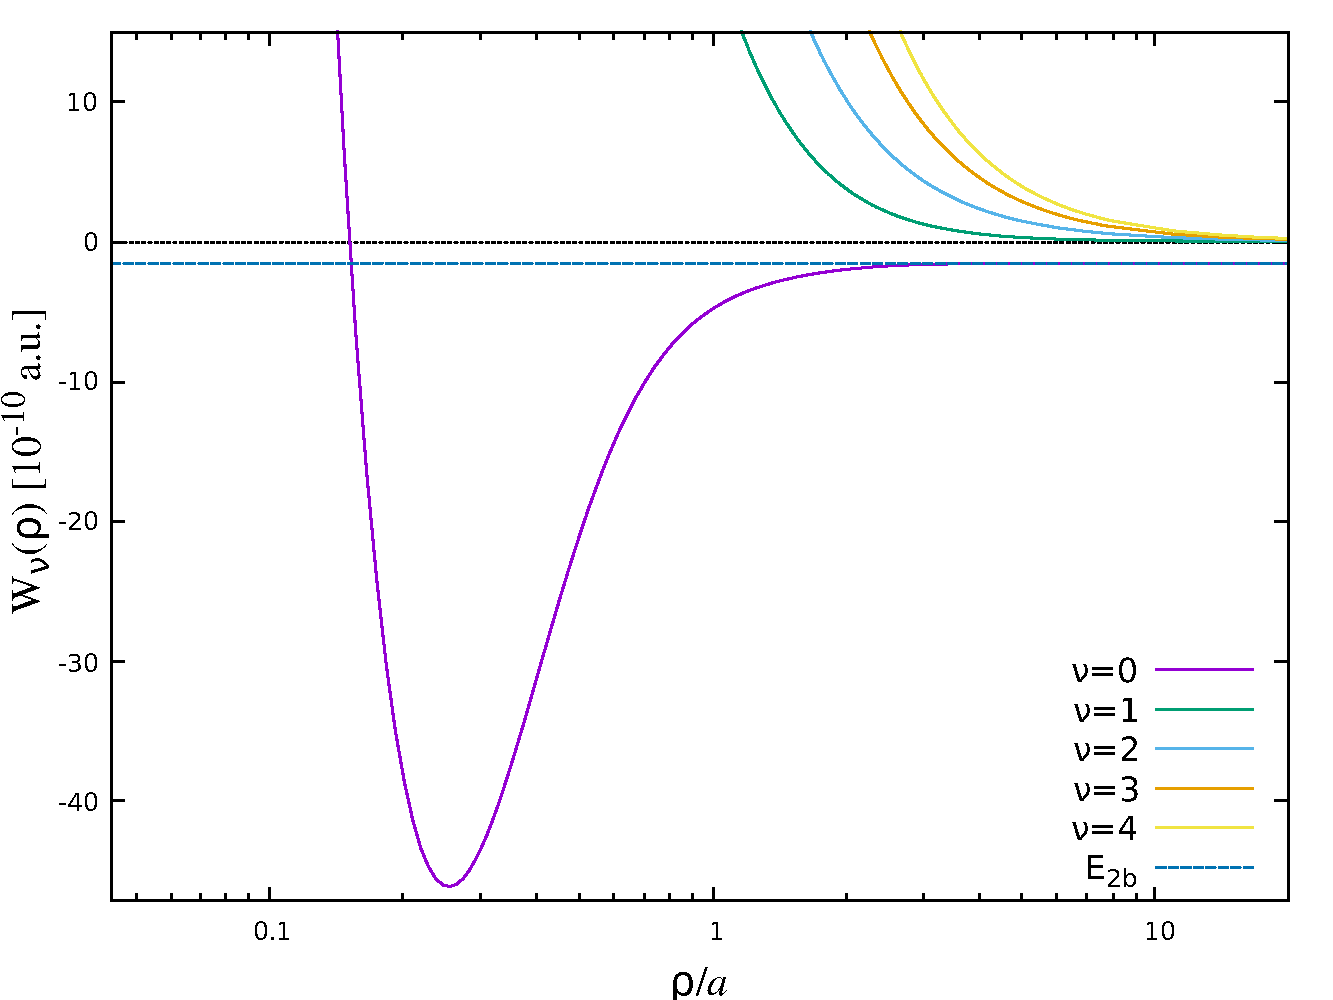
\includegraphics[width=1.0\linewidth]{Wpos.pdf}}
\end{columns}
\end{frame}

\begin{frame}[label=W]
\frametitle{Convergence In the Intermediate Region}
	\visible<1->{\begin{block}{Intermediate Interaction Range}
\begin{equation*}
	r_0 \ll \rho \ll |a|
	\end{equation*}
\end{block}}
	
\visible<2->{\begin{block}{The Lowest Potential's Convergent Form (3 Identical Bosons)}
		\alert<4->{\begin{equation*}\label{eq:efimov_channel}
		W_{\nu}(\rho) = -\frac{s_0^2+\frac{1}{4}}{2\mu \rho^2}
		\end{equation*}} 
\end{block}}

\visible<3->{\begin{block}{Universal Constant (3 Identical Bosons)}
	\begin{equation*}
		s_0 \simeq 1.00624
	\end{equation*}
\end{block}}
\hyperlink{Results}{\beamerbutton{Jump to Results}}
\end{frame}

%------------------------------------------------

\section{Numerical Approach}
\begin{frame}{Numerical Approach; B-spline Collocation}
\only<1>{ 
	\centering
	\huge
	Task = ?}
\only<2>{ 
	\centering
	\huge
	Task = Find \alert<2>{$W_{\nu}(\rho)$}!}
\invisible<-2>{
\parallelcontent
{\begin{description} \item<3->[First:] Find a Basis \end{description}}
{\begin{itemize}\item<4->$\varphi_{lm} = \varphi_{1l}(\theta)\varphi_{2m}(\phi)$\end{itemize}}
\parallelcontent
{\begin{description} \item<5->[Then:] Expand \end{description}}
{\begin{itemize}\item<6->$\Phi_{\nu}(\rho;\theta,\phi) = \sum_{l,m}^{L,M} c_{lm}\varphi_{lm}$\end{itemize}}
\parallelcontent
{\begin{description} \item<7->[Next:] Substitute $\Phi_{\nu}$ into
		\hyperlink<7->{supplemental}{\beamerbutton{Eq. (4)}
		\hypertarget<7->{matrix}}  \end{description}}
{\begin{itemize}\item<8->$\mathbf{H}_{\mathrm{ad}}\mathbf{c} = U\mathbf{B}\mathbf{c}$\end{itemize}}
\parallelcontent
{\begin{description} \item<9->[Finally:] Solve the Generalized Eigenvalue Eq. \end{description}}
{\begin{itemize}\item<10->$W(\rho) = U(\rho)$\end{itemize}}}
\end{frame}

%------------------------------------------------
\section{Scattering Model}
\begin{frame}
\frametitle{Scattering Model}
\begin{columns}
	\column{0.4\textwidth}
\begin{block}<1->{Masses} 
	$m = m(Rubidium-87)$
\end{block}
\begin{block}<2->{Assumption}
	$V(\rho,\theta,\psi) = v(r_{12}) + v(r_{23}) + v(r_{31})$
\end{block}
\begin{block}<3->{2B Model Potential}
	$v(r) = d\cosh^{-2}{(r/r_0)}$
\end{block}
\begin{block}<3->{Interaction Range}
	$r_0 = 55$ a.u.
\end{block}
\column{0.6\textwidth}
%\begin{figure}
	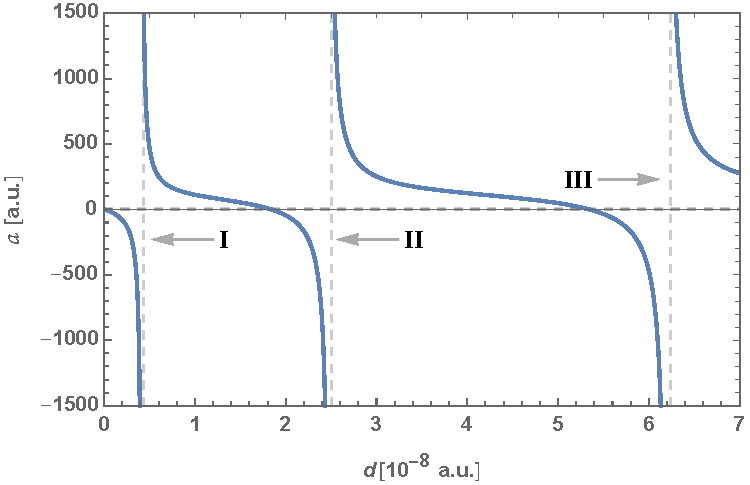
\includegraphics[width=1.0\linewidth]{scattering_new.pdf}
%\end{figure}
\end{columns}
\end{frame}
%------------------------------------------------

\section{Results}
\subsection{Convergence and Accuracy}
\begin{frame}[label=Results]
\frametitle{Convergence and Accuracy}
\begin{itemize}
	\item<1-> For $a \rightarrow \pm \infty$ we expect that the lowest effective potential curve will converge towards
	\hyperlink{W}{\beamerbutton{the Efimovian form}}
	\item This behaviour is easier to recognize if the potentials are multiplied by $2 \mu \rho^2$ and plotted as 
	
	\begin{equation}\label{eq:lambda}
	\xi(\rho) = 2 \mu \rho^2 W_{\nu}(\rho) + \frac{1}{4}
	\end{equation}
	since these curves should approach the universal value $-s_0^2 (\simeq -1.0125$) in the intermediate region
\end{itemize}
\end{frame}


\begin{frame}
\frametitle{$a \rightarrow \pm \infty$, $-s_0^2 (\simeq -1.0125$ for $J=0^+$ states)}
\begin{figure}
	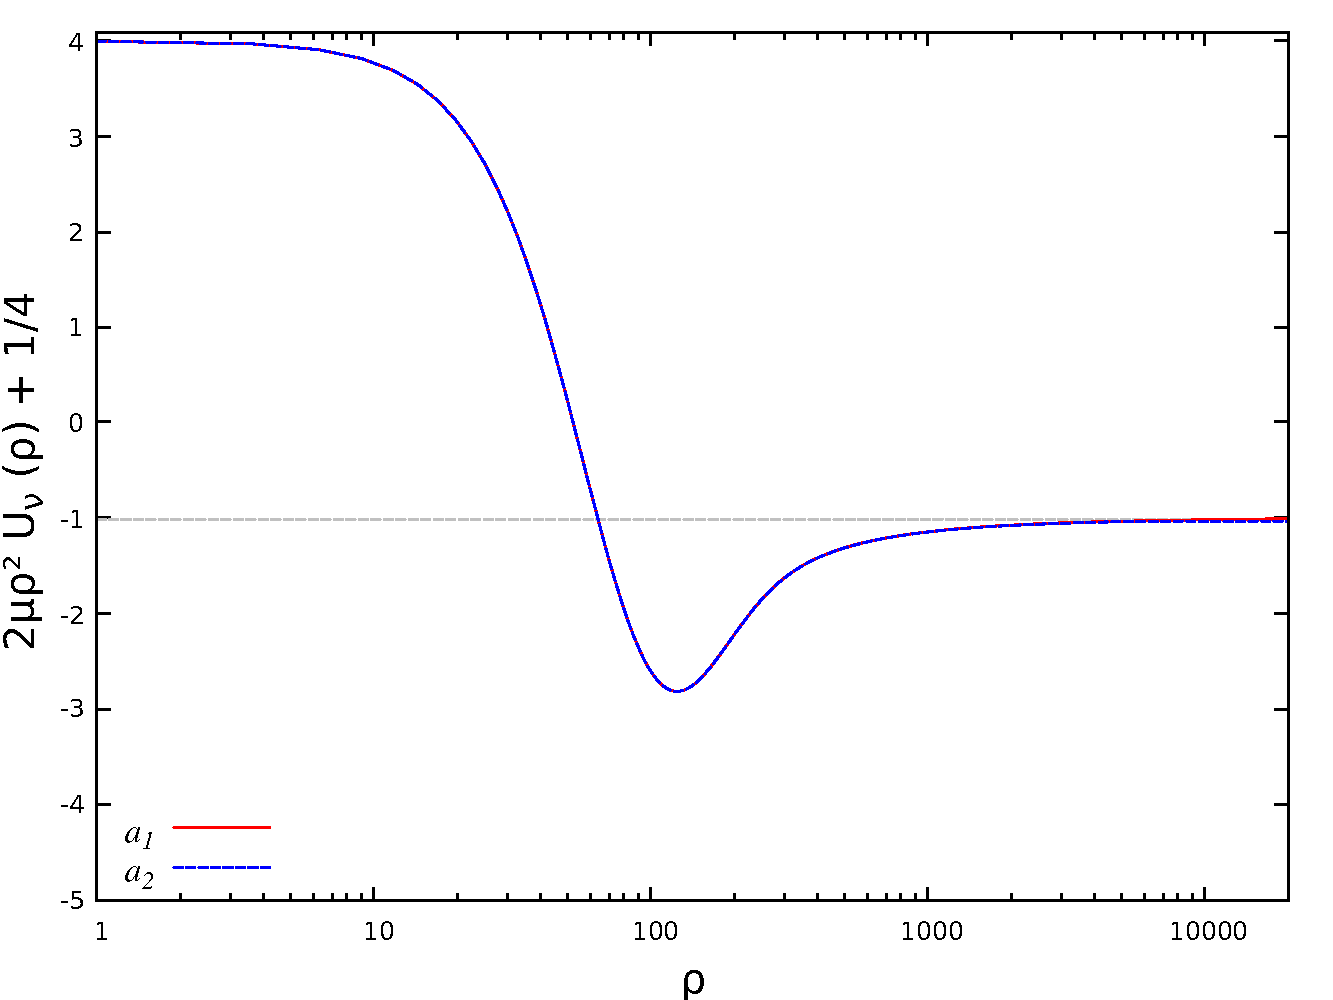
\includegraphics[width=0.8\linewidth]{infty.pdf}
\end{figure}
\end{frame}

\begin{frame}
\frametitle{$a >0$}
\begin{figure}
	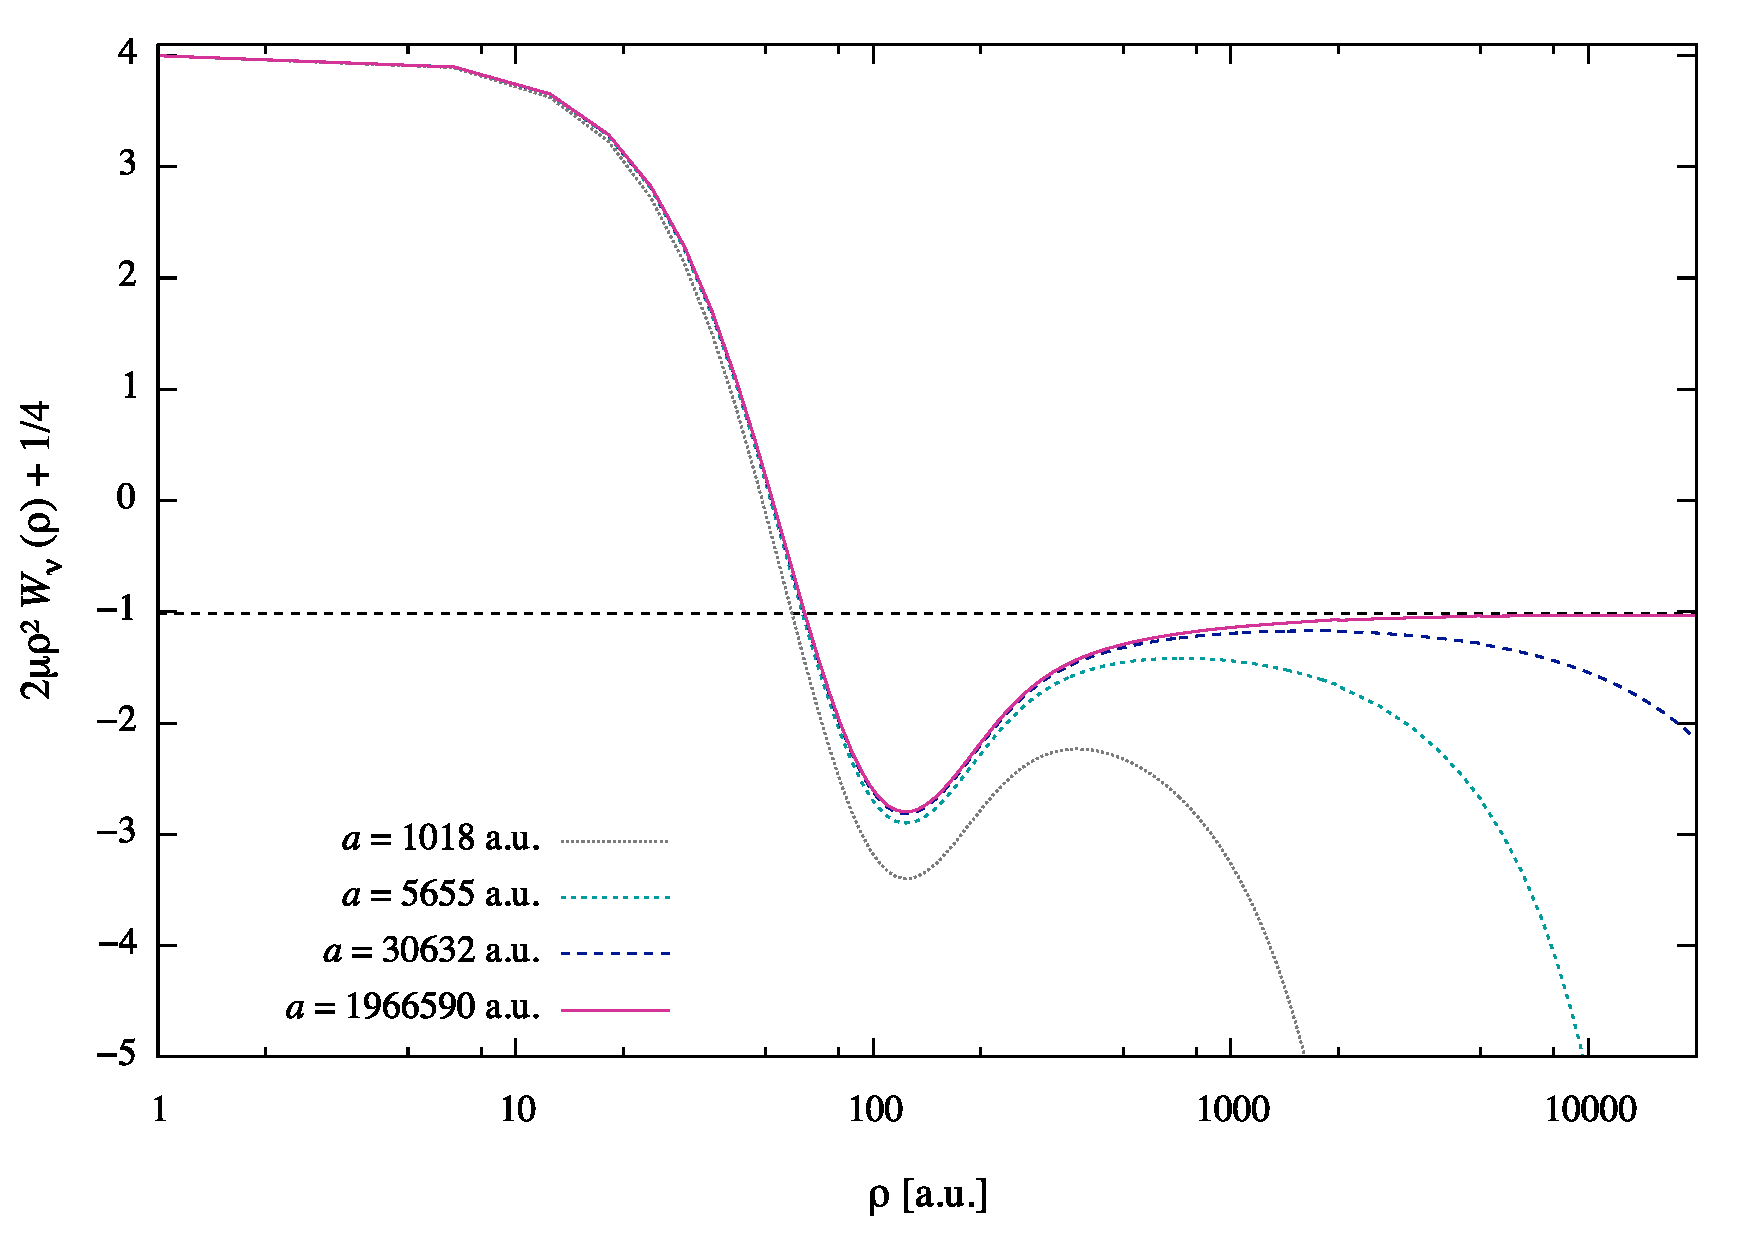
\includegraphics[width=0.8\linewidth]{finite_positive_a.pdf}
\end{figure}
\end{frame}

\begin{frame}
\frametitle{$a<0$}
\begin{figure}
	\begin{figure}
		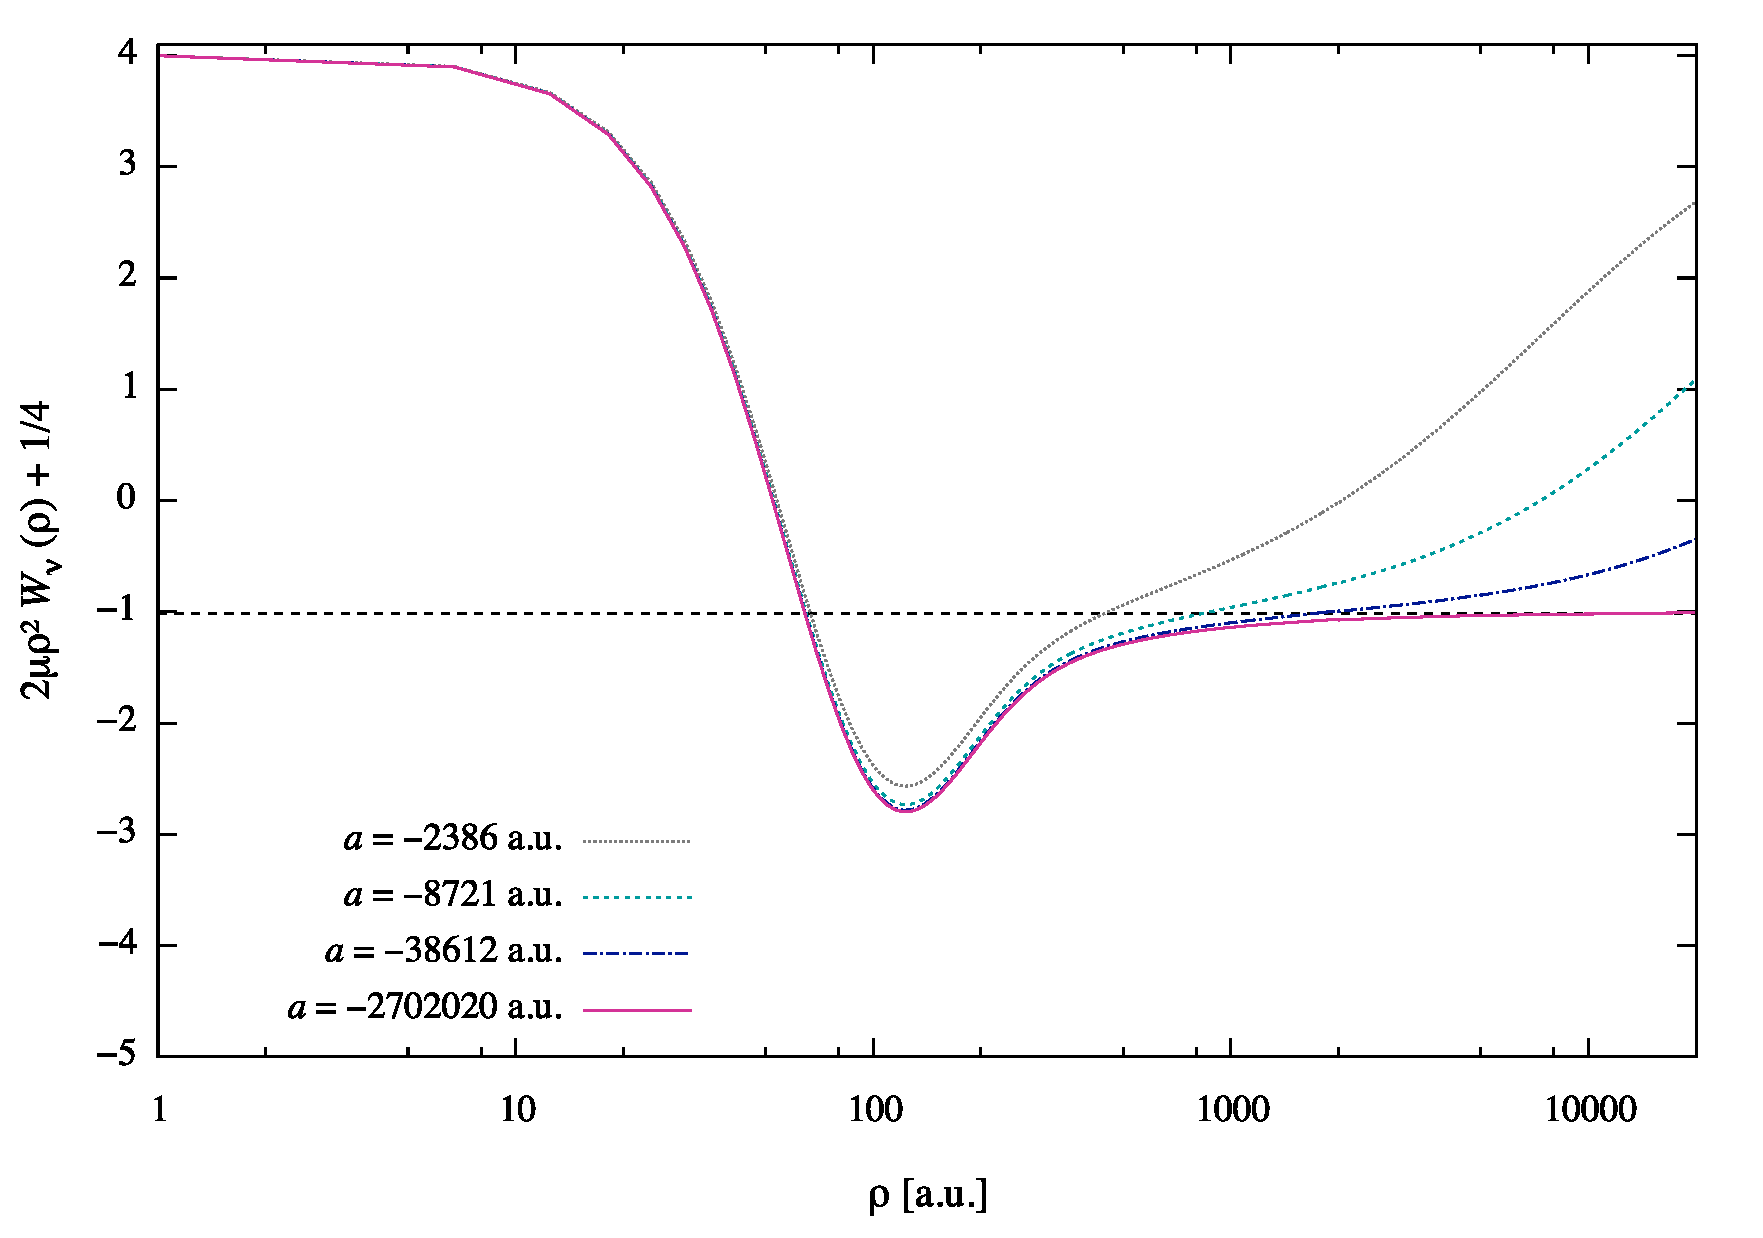
\includegraphics[width=0.8\linewidth]{finite_negative_a.pdf}
	\end{figure}
\end{figure}
\end{frame}

\subsection{Comparison to the Analytical Model}
\begin{frame}
\frametitle{Comparison With the Adiabatic Potential From Solving Faddeev's Equation}
For $\rho \gg r_0$ the adiabatic potentials $\nu_n$ (which correspond to $ \xi(\rho)$) can be determined analytically through the transcendental equation

\begin{equation}\label{eq:transcendental}
\sqrt{\nu_n} \cos{\bigg(\sqrt{\nu_n} \frac{\pi}{2}\bigg)} - \frac{8}{\sqrt{3}}\sin{\bigg(\sqrt{\nu_n} \frac{\pi}{6}\bigg)} = \sqrt{2}\frac{\rho}{a}\sin{\bigg(\sqrt{\nu_n} \frac{\pi}{2}\bigg)}, 
\end{equation}
for different scattering lengths $a$.
\end{frame}

\begin{frame}
\frametitle{Faddeev}
	\begin{figure}
		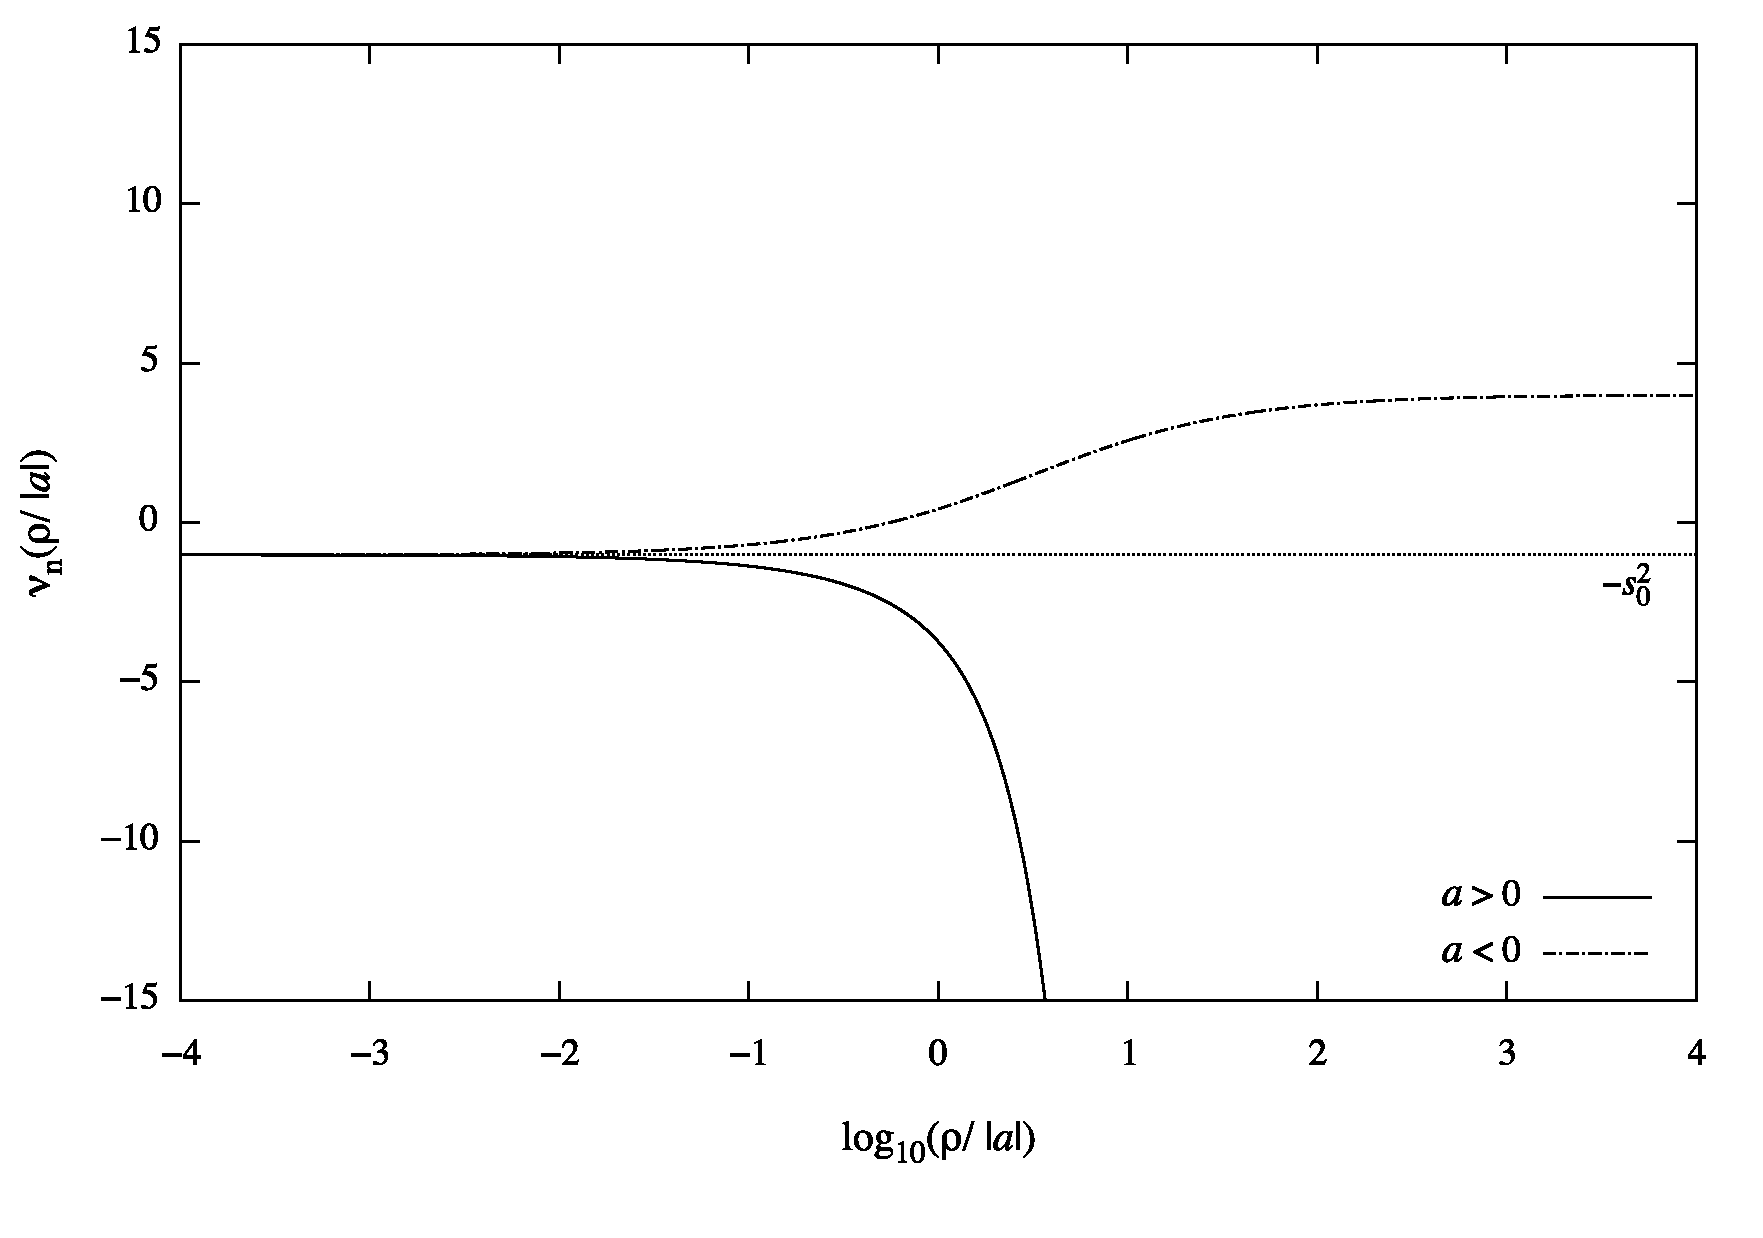
\includegraphics[width=0.8\linewidth]{faddeev.pdf}
	\end{figure}
\end{frame}


%----------------------------------------------------------------------------------------

\end{document} 